\documentclass[letter, 10pt]{article}

\usepackage[spanish]{babel}
\usepackage{amsfonts}
\usepackage{amsmath}
\usepackage[hidelinks]{hyperref}
\usepackage{graphicx}
\usepackage{algorithmic}
\usepackage[noend]{algpseudocode}
\usepackage{algorithm}
\usepackage{url}
\usepackage[utf8]{inputenc}
\usepackage{graphicx}
\usepackage[top=3cm,bottom=3cm,left=3.5cm,right=3.5cm,footskip=1.5cm,headheight=1.5cm,headsep=.5cm,textheight=3cm]{geometry}
\newcommand{\commentsymbol}{//}% or \% or $\triangleright$
\algrenewcommand\algorithmiccomment[1]{\hfill \commentsymbol{} #1}
\makeatletter
\newcommand{\LineComment}[2][\algorithmicindent]{\Statex \hspace{#1}\commentsymbol{} #2}
\makeatother
\newcommand{\varfont}{\texttt}

\begin{document}
\title{Inteligencia Artificial \\ \begin{Large}Estado del Arte: Truck and Trailer Routing Problem\end{Large}}
\author {Matías Vargas}
\date{\today}
\maketitle


%--------------------No borrar esta secci\'on--------------------------------%
\section*{Evaluaci\'on}

\begin{tabular}{ll}
Resumen (5\%): & \underline{\hspace{2cm}} \\
Introducci\'on (5\%):  & \underline{\hspace{2cm}} \\
Definici\'on del Problema (10\%):  & \underline{\hspace{2cm}} \\
Estado del Arte (35\%):  & \underline{\hspace{2cm}} \\
Modelo Matem\'atico (20\%): &  \underline{\hspace{2cm}}\\
Conclusiones (20\%): &  \underline{\hspace{2cm}}\\
Bibliograf\'ia (5\%): & \underline{\hspace{2cm}}\\
 &  \\
\textbf{Nota Final (100\%)}:   & \underline{\hspace{2cm}}
\end{tabular}
%---------------------------------------------------------------------------%
\vspace{2cm}


\begin{abstract}
La finalidad del presente documento es realizar un  análisis del problema TTRP, el cual nace como evolución del problema VRP, considerando aplicaciones más cercanas a la realidad. Este consiste en abastecer un conjunto de clientes con una flota de camiones, los cuales pueden tener un trailer acoplado y el objetivo principal es que cada cliente sea abastecido una única vez y el costo incurrido por la flota sea mínimo. Este problema tiene diversas aplicaciones en la vida real, generalmente es utilizado en problemas donde se deben abastecer clientes y los caminos para llegar a ellos son de difícil acceso, por tanto se decide desacoplar el trailer en una ubicación conveniente y continuar solo con el camión. Al ser un problema interesante en la industria, varios investigadores han decidido abordado  y en este documentos nos centramos en los diferentes enfoques utilizados entre el año 2002 y 2015.
\end{abstract}

\section{Introducci\'on}

\subsection{Propósito y Estructura del documento}
\\
Un problema recurrente en la industria de transporte de cargas, es abastecer la demanda de diferentes clientes en forma óptima. La finalidad es gastar lo menos posible en insumos de transportes (bencina, mantenciones, costos de transportes en general) y además seleccionar el tipo adecuado de transporte, en base a la demanda que se desea abastecer. En base a este contexto surge el problema \textit{Truck and Trailer Routing Problem} (TTRP), el cual será definido en profundidad con la siguiente estructura: En la sección 2, se define el problema y la estructura básica con sus diferentes variantes. En la sección 3, se realizara un estado del arte acerca de TTRP, comenzando desde el año 2002 por Chao\cite{Chao} hasta el año 2015 realizado por Isis\cite{Isis}, presentando las diferentes heurísticas de construcción y reparación de diversos investigadores. En la sección 4, se define en profundidad el modelo matemático del problema. Finalmente, la sección 5 se encuentran los detalles de la representación que se utilizó para resolver el problema y en la sección 6 la descripción del algoritmo, con su explicación a través de pseudocódigos.
\subsection{Descripción del problema y Motivación}
El problema \textit{Truck and trailer routing problem} (TTRP) es introducido por Chao\cite{Chao} en año 2002. Este nace como una variante del problema \textit{Vehicle Routing problem} (VRP), siendo un acercamiento más tangible de la realidad. El problema TTRP consiste en en una flota de vehículos compuesto por $m_{k}$ camiones y $m_{l}$ trailers (compartimientos) que deben servir a un conjunto de clientes y además la cantidad de camiones debe ser mayor a la de trailers. A causa de diversos problemas con las rutas (caminos de difícil acceso) es que se distinguen diferentes tipos de clientes y rutas.\\
La motivación para el estudio de TTRP es el lugar central que ocupa en la administración y logística de distribución, teniendo diversos usos industriales. Gerdessen\cite{Gerdessen} presenta dos aplicaciones de TTRP. La primera es la distribución de productos lácteos por parte de la industria holandesa, en la que muchos clientes se encuentran en ciudades de alto tráfico y estacionamiento limitado. Maniobrar vehículos en estos ambientes es complicado, por lo que deciden dejar el trailer afuera de la ciudad y continuar la entrega de los clientes sin el trailer. \\La segunda aplicación se basa en la entrega de alimentos para animales en diversos graneros, en donde los caminos y puentes son muy estrechos, por lo que hay diferentes tipos de vehículos para transitar.


\section{Definici\'on del Problema}

 El problema que busca resolver TTRP es satisfacer la demanda de todos los clientes con una determinada flota de camiones, los cuales deben empezar y terminar en el mismo depósito. Cada camión debe tener su propia ruta asociada (diferentes tipos de rutas) y los clientes que serán visitados (diferentes tipos de clientes), con la restricción que todos deben ser visitados solo una vez. El objetivo del problema  es minimizar la distancia total recorrida o el costo incurrido de la flota. Para entender el problema hay que  comprender las diferentes componentes que se pueden visualizar en la figura [\ref{fig:Tipos}] extraída del paper de Ulrich \cite{Ulrich}, estas son las siguientes:
 \subsection{Variables del problema}
 \begin{itemize}
     \item En primer lugar se debe solucionar un problema de asignación y la variable binaria utilizada consiste en asignarle a cada cliente $i$ un camión de la flota $j$.
     \item El segundo lugar se debe solucionar el problema de \texttit{TSP} para cada camión y la  variable binaria representa si el camión va del cliente $i$ al cliente $j$.
 \end{itemize}
 \subsection{Tipos de clientes}
 \begin{itemize}
     \item Cliente de vehículo: Puede ser servido por el camión con o sin el trailer.
     \item Cliente de camión: Solo puede ser servido con el camión sin el trailer.
 \end{itemize}
 \subsection{Tipo de rutas}
 \begin{itemize}
     \item Ruta de camión pura: El camión satisface la demanda sin usar el  trailer. Se pueden servir clientes de tipo camión o vehículo.
     \item Ruta de vehículo pura: El camión sirve los clientes con el trailer acoplado. Solo clientes de vehículo son servidos.
     \item Ruta de vehículo completa: El camión debe desacoplar al menos una vez el trailer y estacionarlo en un cliente de tipo vehículo (este trayecto es la ruta principal). Posteriormente, el camión continúa sirviendo un subconjunto de clientes en una sub ruta. Después de servir a todos, el camión debe volver al cliente de vehículo donde estaciono el trailer y finalmente puede realizar otra sub ruta o bien anclar el compartimiento y continuar con la ruta principal.
 \end{itemize}
 \subsection{Particionamiento de la ruta de vehículo completa}
\begin{itemize}
    \item Ruta principal: Es la secuencia de clientes servidos por el vehículo completo.
    \item Sub ruta: Es la secuencia que comienza cuando el camión aparca el trailer en un cliente de vehículo, el cual se conoce como la raíz de la sub ruta. 
\end{itemize}

\subsection{Restricciones}
\begin{itemize}
    \item El cliente puede ser servido solo una vez.
    \item El camión inicia en un depósito y debe finalizar en él.
    \item Las sub rutas pueden sobrepasar la capacidad del camión, solo en el caso que este permitido la transferencia de productos.
    \item La longitud de la ruta recorrida por el vehículo puede estar limitada.
    \item La demanda de ruta vehículo pura y completa no debe superar la capacidad del camión más el compartimiento.
    \item La sub ruta debe comenzar y finalizar en el mismo cliente de vehículo, antes de continuar la ruta principal.
    \item La cantidad de camiones debe ser mayor a la de trailers.
\end{itemize}
\subsection{Paramétros del problema}
\begin{itemize}
    
    \item $n$ es la cantidad de clientes.
    \item $m_{k}$ es la cantidad de camiones.
    \item $m_{l}$ es la cantidad de trailers.
    \item $m_{k}-m_{l}$ es la cantidad de rutas de camión puro.
    \item $c_{ij}$ es el costo asociado a la distancia euclideana entre el cliente $i$ y el cliente $j$.
    \item $q_{i}$ es la demanda del cliente $i$.
    \item $Q_{k} $ y $Q_{l}$ es la capacidad del camión y trailer respectivamente.
    \item El problema puede ser representado mediante un grafo $G=\{V,E\}$, en donde $V=\{1,2,3,...,n\}$ es el conjunto de clientes (0 el depósito) y $E$ es el conjunto de arcos entre los nodos clientes.
    
\end{itemize}

\subsection{Variantes del problema}
\begin{itemize}
    \item Considerar ventanas de tiempos: Esta variante (TTRPTW) considera que los clientes solo aceptan ser servidos durante un periodo de tiempo específico.
    \item Caso en que no se puede desacoplar el trailer y además puede haber más de un deposito (MDTTRP).
    \item Los vehículos no son necesarios que vuelvan al depósito (OTTRP)
    \item Considerar transferencia de productos entre el compartimiento y el camión
    \begin{itemize}
        \item Modelo de Chao \cite{Chao}: Considera transferencia de productos siempre y cuando la recarga no requiera de herramientas o dispositivos que no esté a bordo.
        \item Modelo de Gerdessen \cite{Gerdessen}: Se consideran que los productos se pueden tranfererir, ya que son livianos o líquidos.
        \item Modelo de Ulrich \cite{Ulrich}: No considera transferencia de productos.
    \end{itemize}
    
\end{itemize}
\subsection{Problemas Relacionados}
\begin{itemize}
    \item Vehicle routing problem (VRP): Consiste en una flota de vehículos homogéneo que se distribuyen en diferentes rutas para servir diferentes clientes. Todos deben iniciar en un único depósito. El objetivo es a cada vehículo proveer una secuencia de visitas en la cual todos los clientes sean servidos y la distancia total de viaje por la flota sea mínima. 
    \item Partial Accessibility Constraint VRP (PACVRP): Se asume que todos los camiones disponibles son utilizados y el número de compartimientos necesita ser determinado. Pueden haber cambios en los costos, al considerarse el sueldo de todos los conductores.
    \item VRP con compartimiento (VRPT): Planteado por Gerdessen \cite{Gerdessen}, en donde se realizan dos importantes suposiciones. La primera es que todos los clientes poseen una demanda unitaria. En segundo lugar, cada compartimiento puede ser estacionado solo una vez, es decir, una ruta de vehículo completa con exactamente un sub-tour. Gracias a esto último, no es necesario considerar costos de estacionamiento y desacoplamiento del compartimiento.
\end{itemize}
\begin{figure}[h]
    \centering
    \caption{Esquema del problema TTRP}
    \vspace{0.5cm}
    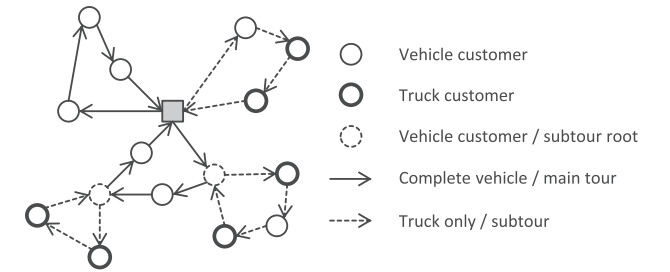
\includegraphics[scale=0.8]{Images/Tipos.png}
    \label{fig:Tipos}
\end{figure} 

\section{Estado del Arte}
En las siguientes subsecciones, se realizara un análisis completo sobre el estado del arte del problema TTRP, con las diferentes heurísticas y métodos que se han utilizado para la resolución del problema, estas serán presentadas en orden cronológico. 


\subsection{Descent improvement steps}
     En el año 2002 Chao~\cite{Chao} desarrollo las bases del problema, considerando una heurística de mejora de soluciones que es conocida como \textit{Descent Improvement steps} para el problema \textit{TTRP}. Consiste en que los clientes son asignados a una de los tres tipos de rutas, a través de resolver un problema de asignación. Posteriormente, se intenta cambiar a los clientes a una nueva ruta, con el objetivo de convertir una solución que previamente era infactible en una factible. La estrategia es considerar una penalidad $\theta$ que mida el grado de infactibilidad de este cambio. Se considera una penalidad de la ruta R ($\theta_{R}$), la cual es computada como $\theta_{R} = max(0, \alpha_{R}-\Gamma_{R})$, en donde $\alpha_{R}$ es la demanda de la ruta R y $\Gamma_{R}$ es la capacidad del camión de R.
        \\
        \begin{enumerate}
            \item\textit{One-point descent movement}: La finalidad es mover un cliente de una ruta a otra. Si el movimiento candidato decrementa la penalidad con o sin un aumento de distancia, o bien disminuye la distancia sin aumentar la penalidad, entonces se ejecuta inmediatamente el cambio. Hay dos movimientos que deben ser excluidos: El primero es mover un cliente de camión a un tour principal perteneciente a una ruta de vehículo completa, o bien a una ruta de vehículo pura. La segunda es mover un cliente de vehículo, que es el estacionamiento de un sub-tour (cliente raíz). 
            \\
            \item\textit{Two-point descent exchange}: Dos clientes de dos rutas diferentes pueden ser intercambiados. Considerándose las mismas restricciones que el caso anterior.
            \\
            \item\textit{ Sub-tour root-rexning step}: En los casos anteriores los nodos raíces no cambiaron su posición, sin embargo es posible que el cambio genere una mejor solución. En este paso se intenta intercambiar los nodos raíces y hacer una posible re secuencia de las sub rutas, eliminando el primer y último arco que llega al nodo raíz y probar otras combinaciones, con otro nodo raíz. Este proceso se puede apreciar en la imagen [\ref{fig:Root}].
        \end{enumerate}
        
    \begin{figure}[h]
    \centering
    \caption{Paso de refinamiento de un nodo raíz}
    \vspace{0.5cm}
    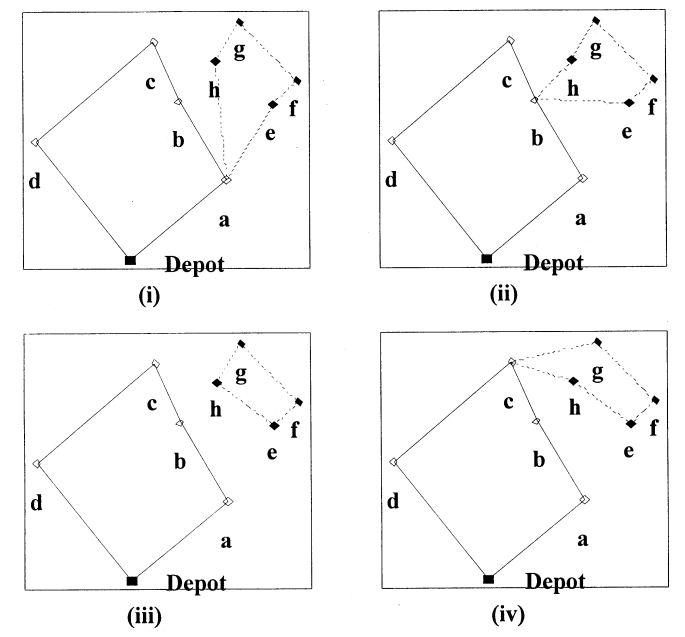
\includegraphics[scale=0.4]{Images/Root.png}
    \label{fig:Root}
    \end{figure}
    \\
   Chao resolvio 21 instancias del problema  [\ref{fig:Instancias}]. Estas se consolidaron como las bases para los investigadores posteriores, siendo los casos de comparación.

\begin{figure}[h]
    \centering
    \caption{Instancias de problema TTRP diseñadas por Chao}
    \vspace{0.5cm}
    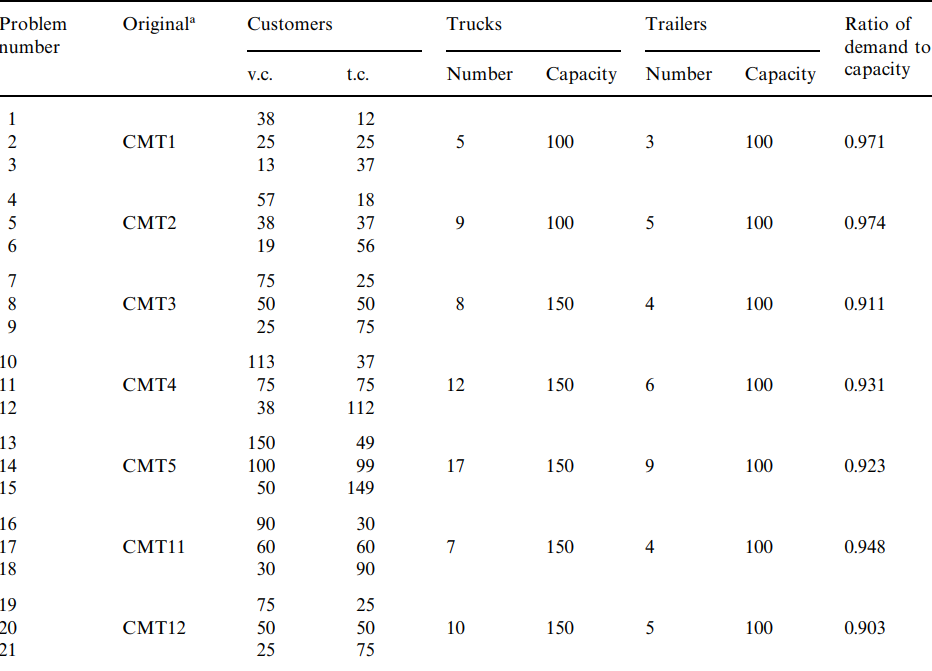
\includegraphics[scale=0.6]{Images/Instancias.png}
    \label{fig:Instancias}
\end{figure}

\newpage
\\
\subsection{Tabu Search}\\ 
\\
Esta es una heurística de mejora basada en realizar búsquedas locales, siendo ampliamente utilizado en problemas de optimización combinatorial. Sirve para guiar la búsqueda  y evitar quedarse atrapado en óptimos locales, moviéndose en cada iteración de una solución S a la mejor solución vecina posible  S'. Para evitar las búsquedas cíclicas, las soluciones visitadas recientemente que cumplen un determinado atributo se memorizan en una lista tabú (restricción tabú) durante un número de iteraciones.  Las soluciones vecinas de S que contienen tal atributo se consideran temporalmente tabú o prohibidas, a menos que cumplan con el llamado criterio de aspiración.
\\
\\
Dentro del mismo año 2002, Chao~\cite{Chao}, en su paper utiliza el método \textit{Tabu Search}, proponiendo dos restricciones tabús: La primera es \textit{FTB}, la cual prohíbe que un cliente vuelva a una ruta del que fue eliminado en las últimas $\pi$ iteraciones. La segunda restricción es OTB (objective-based value) y hace uso del concepto \textit{Deterministic annealing}. Este último consiste en solo considerar soluciones con valores de la función objetivo que están dentro de una cantidad específica (desviación) del mejor valor de la función objetivo hasta el momento.  Una solución candidata con un valor de la función objetivo mayor que el mejor valor de la función objetivo más una desviación estará prohibida como restricción tabú.
Por otra parte,  usa un criterio de aspiración que anula la restricción tabú cada vez que una solución candidata produce un valor de función objetivo que es menor que el mejor valor actual.

\subsection{T-Cluster and T-Sweep}
En el año 2006, Scheuerer~\cite{Scheuerer} propone la utilización de dos heurísticas de construcción, para la mejora de los resultados obtenidos por Chao.\\ En primer lugar se encuentra \texttit{T-Cluster}, este es considerado como un procedimiento de inserción secuencial basado en grupos, donde las rutas se construyen cliente a cliente hasta la utilización total de la capacidad del vehículo. Se inicializa una nueva ruta con el cliente sin ruta más alejado del depósito y el vehículo no utilizado que tiene la capacidad total máxima. En el caso de que sea un vehículo completo, si el cliente inicial es de vehículo, entonces se inserta en el recorrido principal y si es de camión se insertara en un nuevo sub recorrido. El siguiente cliente para ser insertado en la ruta es minimizando la siguiente ecuación: $e(k) = c_{ku}+ c_{kf}-\pi c_{0k}$, donde $k$ especifica el cliente en consideración, $f$ es el cliente más cercano enrutado en esta ruta y 0 el depósito. El término $c_{ku}$ mide la distancia del cliente inicial de la ruta u y el cliente en consideración k. Esta distancia se debe mantener mínima para garantizar la compactitud de la ruta. El segundo término $c_{kf}$ asegura que está cerca del "borde" de la ruta actual. Finalmente el térmico $\pi c_{0k}$ es conocido como el término de diversificación, en donde la variación del parámetro $\pi$ resultara en la selección de una nueva estrategia.
\\\\
En segundo lugar se encuentra \texttit{T-Sweep} presentado en la figura [\ref{fig:sweep}], es un heurística basada en el clásico algoritmo \textit{Sweep} atribuido a Gillett y Miller \cite{Gillett}. Esta técnica de barrido es utilizada para constuir soluciones factibles girando un rayo centrado en el depósito e incluyendo gradualmente a los clientes en una ruta de vehículos. Se inicializa una nueva ruta con el vehículo no utilizado que tiene la capacidad total máxima, siempre que se alcance la capacidad total del vehículo o la restricción de longitud de la ruta. Si no hay más vehículos disponibles, se permite que la última ruta se vuelva inviable.

\begin{figure}[h]
    \centering
    \caption{Ejemplo de T-Sweep}
    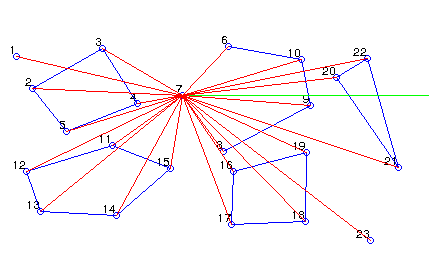
\includegraphics[scale=0.5]{Images/sweep.png}
    \label{fig:sweep}
\end{figure}
\\
Finalemente, Scheuerer \cite{Scheuerer} también utiliza  la heurística de \textit{Tabu Search}, pero con nuevas mejoras. En la figura [\ref{fig:tabla}] se puede ver que las soluciones encontradas por Scheuerer son mejores para las 21 instancias de Chao, en donde $c(s^{*})$ representa la distancia total, $q(s^{*})$ la sobrecapacidad total y T el tiempo total, en segundos.
\begin{figure}[h]
    \centering
    \caption{Comparación de soluciones entre Chao y Scheurer}
    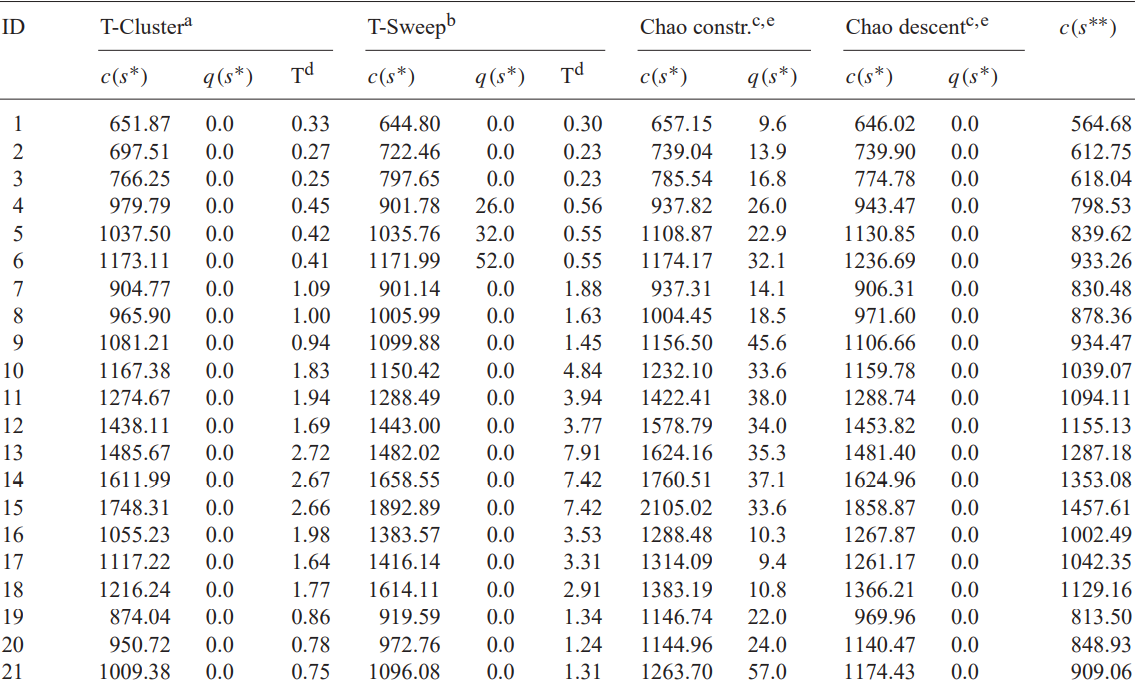
\includegraphics[scale=0.6]{Images/Chao-Scheurer.png}
    \label{fig:tabla}
\end{figure}
\newpage
\subsection{Simulated Annealing}
Shih-Wei Lin~\cite{Lin} en el año 2009 propone la utilización de una heurística llamada \textit{Simulated annealing} para resolver el problema de TTRP. Esta es una heuristica de búsqueda local capaz de escapar de un óptimo local, aceptando en pequeña probabilidad peores soluciones durante ciertas iteraciones. El concepto de annealing hace alusión a lograr un cercano mínimo global imitando el enfriamiento lento producido en el proceso físico de recocido de los metales. Este comienza con una solución inicial aleatoria y en cada iteración el algoritmo toma una nueva solución de la vecindad predefinida en la solución actual. El valor de la función objetivo de la nueva solución es comparado con la solución actual y en caso que sea mejor, se reemplaza la solución actual.
\\Shih-Wei Lin \cite{Lin} mezcla este método con una búsqueda aleatoria de vecindad que presenta varios tipos de movimientos. Para la inserción establece seleccionar un cliente aleatorio i de la solución S e insertarlo en la posición precedente de otro cliente aleatorio j de la solución S. Por otro lado, el intercambio es seleccionando aleatoriamente el cliente x y j de la solución S, para luego intercambiarlos. Finalmente cambiar el tipo de vehículo es seleccionando aleatoriamente un cliente de vehículo y cambiar el servicio a tipo camión o vice versa.\\
\\
Es importante destacar que Lin en el año 2011 resuelve instancias para el problema TTRPTW (TTRP con ventanas de tiempo), siendo el primero en resolverlo.\\\\
En la figura[\ref{fig:Lin}] se puede apreciar la comaparación entre Lin, Chao y Scheuerer. En donde pudo obtener 17 mejores soluciones de los 21 problemas y 4 instancias continuaron con mejor solución para Scheurer, sin embargo el tiempo de ejecución de Lin fue el mejor en todos los casos. $c(s^{*})$ representa la distancia total y T el tiempo de ejecución en segundos.

\begin{figure}[h]
    \centering
    \caption{Comparación entre Lin, Chao y Scheurer}
    \vspace{0.5cm}
    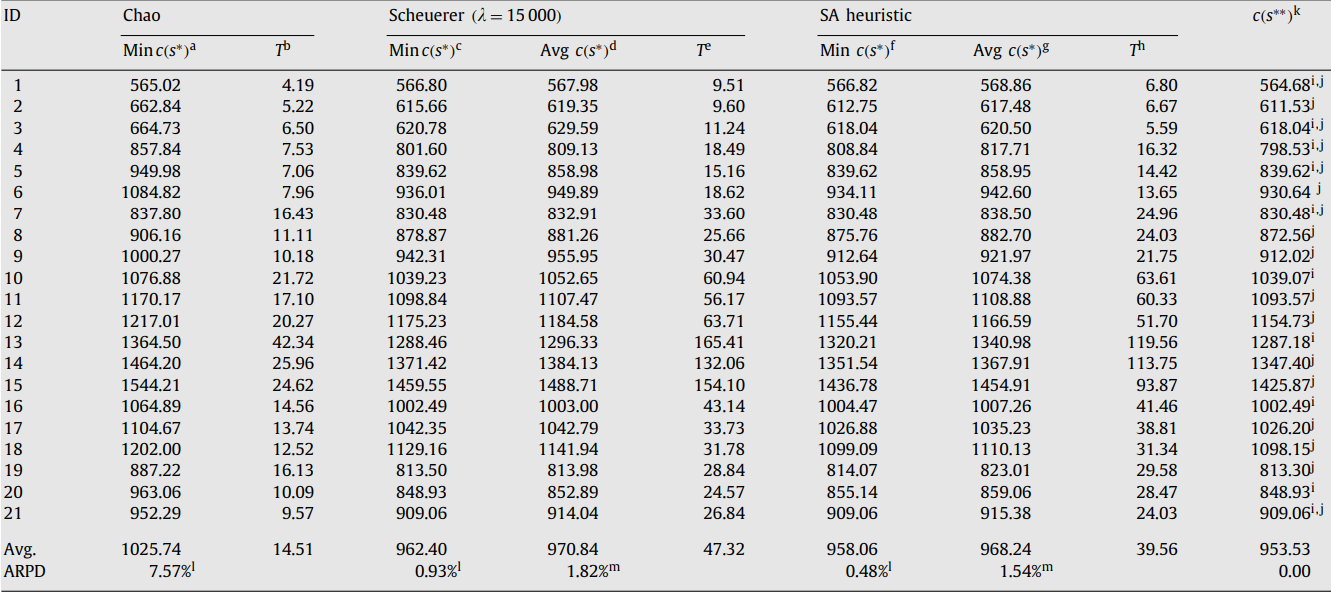
\includegraphics[scale=0.54]{Images/Lin.png}
    \label{fig:Lin}
\end{figure}
\newpage
\subsection{GRASP and VNS}
En el año 2011, Villegas~\cite{Villegas}, introduce una forma para resolver el problema, basado en \textit{Greedy Randomized Adaptive Search Procedure} (GRSAP), \textit{Variable Neighborhood Search} (VNS). En primer lugar GRSAP, es un metaheurística de inicio múltiple sin memoria, que consiste en iteraciones compuestas para la construcción de una solución aleatoria codiciosa y mejoras iterativas de la misma a través de una búsqueda local. Por otra parte, VNS es un método de búsqueda que explora vecindarios distantes de la solución actual a través de dos fases, la primera es de descenso para encontrar un óptimo local y la segunda es una fase de perturbación para salir del valle.
\\
\\
En al figura [\ref{fig:Villegas}] se pueden apreciar las comparaciones entre Villegas y los investigadores anteriores. El estudio de Villegas encontró 11 mejores soluciones.\\ En la figura [\ref{fig:grafico}] se pueden apreciar la mejora en los tiempos de computación, para instancias de 50 clientes hasta 200.

\begin{figure}[h]
    \centering
    \caption{Comparación entre Villegas, Lin, Chao y Scheurer}
    \vspace{0.5cm}
    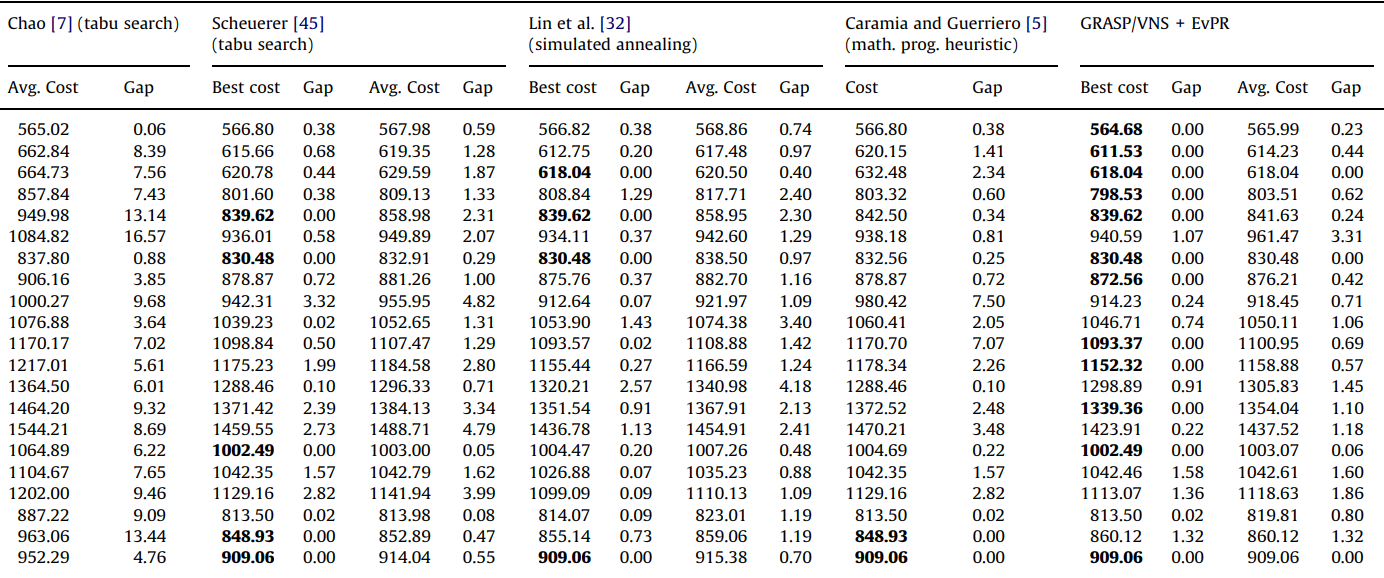
\includegraphics[scale=0.53]{Images/ComVillegas.png}
    \label{fig:Villegas}
\end{figure}
\begin{figure}[h]
    \centering
    \caption{Gráfico de tiempos comparativo entre Villegas, Lin, Scheuerer}
    \vspace{0.5cm}
    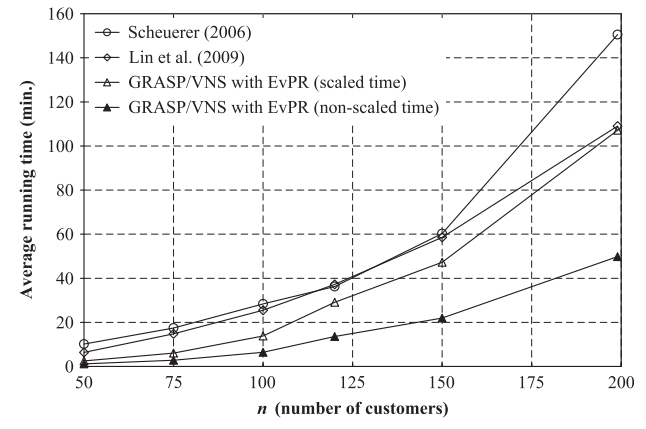
\includegraphics[scale=0.53]{Images/Grafico.png}
    \label{fig:grafico}
\end{figure}

\newpage
\subsection{LS-ABHC, LS-RRT and LNS-RRT}
En el año 2012, Ulrich \cite{Ulrich} propone un enfoque de dos fases. En primer lugar, crear una solución inicial factible basada en búsqueda de vecindarios, \textit{Local search} y \textit{Large Neigborhood Search} (LNS). La segunda fase, se consolida en que los movimientos son aplicados en base a dos metaurísticas de control, \textit{Record-to-Record Travel} (RRT) y \textit{Attribute Based Hill Climber} (ABHC).
\begin{enumerate}
    \item \textit{Local Search}: Se basa en pequeños modificaciones a la solución, siendo su fuerte la intensificación de la búsqueda. Se consideran una serie de movimientos, como, intercambiar o relocalizar. Se puede habilitar la transferencia de sub-tours completos considerando la selección de un nuevo cliente raíz del sub-tour y también se puede cambiar la selección de clientes dentro del sub-tour. Otro tipo de cambio es  clientes de vehículo completo a clientes de camión.\\
    \item \textit{Large neighborhood search}: El concepto de neighborhood se basa en arruinar y recrear. En el problema de TTRP, se aplica el paso de arruinar cuando se remueven una cantidad de clientes de una ruta, los cuales no son servidos temporalmente y el paso de recreación es cuando se re insertan esos clientes de nuevo en la solución con una heurística de inserción barata. En LNS el paso de destrucción es en base a la selección de clientes que son similares respecto a sus distancias.
    \\
    \item \textit{Record-to-record travel}: Se basa en utilizar el costo de la mejor solución encontrada hasta ahora, con la finalidad de definir la ''aceptabilidad" de la solución. El vecino seleccionado (aleatoriamente) es aceptado si no es peor que la mejor solución encontrada hasta el momento por una desviación estándar.
    \\
    \item \texttit{Attribute based hill climber:} Es un tipo de \textit{Tabu Search}, que utiliza atributos genéricos para especificar vecinos no tabú, el cual debe ser especializado para el dominio de cada problema.
\end{enumerate}
La resolución de Ulrich \cite{Ulrich} logro encontrar 18 mejores nuevas soluciones en comparación a Villegas \cite{Villegas}, encontrándose entre los mejores resultados del momento.\\
\subsection{Fuzzy Constraints}
En el año 2015, Torres \cite{Isis} resuelve el problema con un enfoque de \textit{Fuzzy Constraints}. La finalidad es tener un marcador de tolerancia de violación de las restricciones, este marcador permite que las restricciones sean satisfechas tanto como sean posibles. También menciona un enfoque paramétrico, definiendo un valor $\alpha$ que representa el marcador de nivel de satisfacción, en donde todas las restricciones son acotadas a este valor. Probando con diferentes $\alpha$ se encuentra con un conjunto de soluciones. 
\subsection{Tendencia}
Los métodos propuestos por \cite{Ulrich} y Villegas \cite{Villegas} son los que estan funcionando mejor actualmente y son el estado del arte. Por un lado Ulrich, tiene 18 mejores soluciones y utiliza las heurísticas \textit{LS-ABHC, LS-RRT and LNS-RRT}. Por otro lado, Villegas tiene 4 mejores soluciones utilizando las heurísticas de \textit{GRASP and VNS}. 
\newpage

\section{Modelo Matem\'atico}

El modelo matemático que se presentara es planteado por el investigador Chao \cite{Chao}. Se debe solucionar un problema de asignación relajado, en donde a cada cliente se le asigna un camión de la flota que cumplirá su demanda.\\\\\textbf{Paramétros}:
\begin{itemize}
    \item $n$ es la cantidad de clientes.
    \item $m_{k}$ es la cantidad de camiones.
    \item $m_{l}$ es la cantidad de trailers.
    \item $q_{i}$ es la demanda del cliente $i$.
    \item $Q_{l}$ es la capacidad del trailer $l$.
    \item $Q_{k}$ es la capacidad del camión $k$.
    \item $i=1, 2,...,n$. Representa el cliente número $i$.
    \item $j= 1, 2,...,m_{k}$. Representa el camión número $j$.
    \item $d_{ij} = c_{0i} + c_{is_{j}} - c_{0s_{j}}$ representa el costo de asignarle al cliente $i$ el camión $j$. Por otra parte, $s_{j}$ se conoce como un cliente semilla para el camión $j$. La forma de obtenerlo es a través de realizar un proceso iterativo. En la primera iteración, la semilla es el cliente más lejano del depósito, en la segunda iteración el cliente semilla es el más lejano a las semillas precedentes y el depósitos. Se repite este proceso 10 veces encontrando diferentes soluciones iniciales, la última es la mejor.
\end{itemize}
\\
\\
\textbf{Variables}:
\begin{itemize}
    \item $x_{ij}=\{0,1\}$. Es la variable binaria que representa si al cliente $i$ se le asigna el camión $j$.
\end{itemize}
\\
\textbf{Función objetivo}:

\\
\begin{equation}
    min \sum_{i = 1}^{n} \sum_{j = 1}^{m_{k}} d_{ij} x_{ij} \\
\end{equation}
\textbf{Restricciones}:
\\
\begin{equation}
    s.t.  \sum_{j = 1}^{m_{k}} x_{ij} = 1, \quad i=1, 2,...,n
\end{equation}
\begin{equation}
   \sum_{i = 1}^{n} q_{i}x_{ij} \leq Q_{l} + Q_{k}, \quad  j= 1, 2,...,m_{l}
\end{equation}
\begin{equation}
    \sum_{i = 1}^{n} q_{i}x_{ij} \leq Q_{k}, \quad j= m_{l}+1,...,m_{k} 
\end{equation}
\begin{equation}
   0 \leq x_{ij},\quad i=1, 2,...,n, \quad j= m_{l}+1,...,m_{k} 
\end{equation}
\\
\begin{itemize}
    \item La ecuación (1) plantea minimizar el costo total de asignamiento.
    \item Ecuación (2) establece la restricción que ningún cliente tenga asignado más de un camión.
    \item La restricción (3) fuerza que la máxima demanda de una ruta vehículo pura o completa sea menor o igual que la suma de la capacidad del camión y el trailer.
    \item La restricción (4) fuerza que la maxima demanda de cada ruta de camión debe ser menor o igual a la capacidad del camión.
    \item La restricción (5) fuerza a que los $x_{ij}$ tomen valores en el intervalo cerrado $[0,1]$
    \item El espacio de búsqueda es $2^{n*m_{k}}$.
\end{itemize}
Chao\cite{Chao} menciona que pueden haber clientes que tienen asignados valores fraccionarios, en ese caso hay que aproximar el valor a 1. Esto puede generar soluciones infactibles en base a la capacidad de los camiones, sin embargo debe ser solucionado con la heurística de mejora. Para este paso la única finalidad es asignar a los camiones los diferentes clientes.\\ \\
Luego de resolver el problema de asignación, se debe construir las rutas de los camiones con los clientes asignados. Esta parte del problema se soluciona como el problema del vendedor viajero (TSP).
\\\\\textbf{Paramétros}:

\begin{itemize}

    \item $c_{ij}$ es el costo de ir del cliente $i$ al cliente $j$.
    \item Q es el conjunto de recorridos posibles.
\end{itemize} 
\\
\textbf{Variables:}
\begin{itemize}
    \item $x_{ij} =\{0,1\}$. Es la variable binaria que representa si el camión va del cliente $i$ al cliente $j$. 
\end{itemize}
\
\textbf{Función objetivo:}
\begin{equation}
    min \sum_{i = 1}^{n}\sum_{j \neq i, j = 1}^{n} c_{ij}x_{ij}
\end{equation}
\textbf{Restricciones:}
\begin{equation}
    \sum_{i = 1, i \neq j}^{n} x_{ij} = 1, \quad j = 1,...,n
\end{equation}
\begin{equation}
    \sum_{j = 1, j \neq i}^{n} x_{ij} = 1, \quad i = 1,...,n
\end{equation}
\begin{equation}
    \sum_{i\in Q}\sum_{j \neq i, j\in Q} x_{ij} \leq |Q| - 1 , \quad \forall Q \subset \{1,...,n\}, \quad  |Q|\geq 2
\end{equation}
\\
\begin{itemize}
    \item La función objetivo en (6) busca minimizar el costo total de la ruta.
    \item La restricción (7) y (8) establecen que un cliente solo puede ser visitado una vez (del nodo cliente entra un arco y sale un único arco)
    \item La restricción (9) establece que no deben haber sub-recorridos, debe ser la unión de un único recorrido.
    \item El espacio de búsqueda es $(n-1)!/2$.
\end{itemize}
\\
Las rutas de camión y vehículo pura son tratados rápidamente como TSP. En las rutas de vehículo completas, se construye primero la ruta principal y luego el sub recorrido, en donde se puede anidar a otro sub recorrido o comenzar uno nuevo uniéndolo a un cliente de la ruta principal.
\includegraphics[scale=0.53]{image}
\newpage

\section{Representaci\'on}
Para la representación se utilizaron estructuras de C++ y vectores que son equivalentes a arreglos dinámicos con la ventaja de tener varios métodos disponibles para ser utilizados. A continuación se puede ver las estructuras para la asignación de rutas, crear la ruta de tsp y una estructura espacial para las subrutas. 

\begin{verbatim}
typedef struct ASSIGNMENT_ROUTE{   
    float id_semilla;
    float tipo_transporte;
    float demanda_total;
    float cantidad_demandada;
    float capacidad_total;
    float capacidad_disponible;
    vector<int> clientes;
    
} Route;

typedef struct ROUTETSP{
  vector<int> clientes;
  string type;
  float distance;
} RouteTSP;

typedef struct TruckSub{
  vector<int> id_clients;
  int id_ruta;
  float distance;
} TruckSub;
\end{verbatim}
Al momento de resolver el problema de asignación se creara un vector de estructuras \textit{assigment\_route} que contiene los clientes que fueron asignados a cada camión, estos clientes deben satisfacer la capacidad del camión y tráiler según corresponda (cabe mencionar que solo estan los clientes asignados pero aún no se inicia una ruta óptima). La variable tipo\_transporte es 0 si esa ruta no tiene un tráiler acoplado y 1 en caso contrario. También hay variables para guardar la demanda total que se ha satisfecho y la capacidad disponible que tiene el camión para abastecer al momento que se busca asignarle nuevos clientes.\\\\
Luego de ser asignados los clientes a una ruta se debe establecer el camino óptimo resolviendo un problema de \textit{TSP}. Para esto, habrá un vector de estructuras \textit{routetsp} que contiene la secuencia de los clientes, sin embargo, solo se consideran maintours en rutas completas o rutas vehículo puro y además variable distancia, guarda la distancia total de la ruta.
\\ \\
Finalmente, se crea un vector de estructuras \textit{TruckSub} que se encarga de guardar los clientes de las subrutas y tiene como variable un id\_ruta para reconocer a que ruta pertenece.\\\\
Como se puede apreciar, estas representaciones son bastante intuitivas para establecer la relación con el modelo matemático, en donde se pueden manejar restricciones fácilmente, como que un cliente se puede encontrar una única vez en la lista de clientes o que podemos guardar la relación capacidad disponible del camión para saber si podrá satisfacer un nuevo cliente que se busca asignarle, de esta forma satisfacemos las restricciones de oferta/demanda.
\section{Descripci\'on del algoritmo}
Para resolver el problema TTRP se utilizó el enfoque propuesto por Chao \cite{Chao}. En primer lugar se debe resolver el problema de asignación y para esto, debemos crear semillas (cada semilla es un cliente particular de una ruta) y asignarle una a cada camión. El proceso de generación de semillas es el siguiente:
\begin{itemize}
    \item La primera semilla es la más lejana del depósito.
    \item La segunda semilla es la más lejana del deposito y de la primera semilla.
    \item La semilla n es la más lejana del depósito y de las n-1 semillas precedentes.
\end{itemize}

Para encontrar las semillas, en primer lugar debemos crear una matriz de distancias de dimensiones $(n+1)$x$(n+1)$ (n es la cantidad de clientes y +1 porque se incluye las distancias del depósito), esta matriz contiene las distancias entre todos los clientes y además es simétrica.\\
Después de ser asignada cada semilla a cada ruta, se deben comenzar a asignar los clientes. Para esto se creó un algoritmo greedy que busca asignar a cada cliente la ruta de semilla $s_{j}$ que tenga menor costo $d_{ij}$. En nuestro problema el costo es simplemente la distancia y este valor se calcula como:
\begin{center}
    $d_{ij} = c_{0i} + c_{is_{j}} - c_{0s_{j}}$
\end{center}
\begin{itemize}
    \item $d_{ij}$ costo de asignarle al cliente $i$ el camión $j$.
    \item $s_{j}$ es el cliente semilla para el camión $j$.
    \item $c_{0i}$ es el costo del depósito al cliente i.
    \item $c_{is_{j}}$ es el costo del cliente i a la semilla $s_{j}$.
    \item $c_{0s_{j}}$ es el costo del depósito a la semilla $s_{j}$.
\end{itemize}
También se debe calcular una matriz de distancias de $c_{is_{j}}$ (de los clientes a las semillas), para que el algoritmo greedy pueda seleccionar la menor distancia en esta matriz, la cual tendrá dimensiones de n x nCamiones.\\
A continuación se detallará el algoritmo en pseudocódigo:\\
\begin{algorithm}[H]
\begin{algorithmic}
    \LineComment[0\dimexpr\algorithmicindent]{\textit{Cada nodo representa un cliente con propiedades de (id,x,y,demanda,tipo)}}
    \STATE{\textbf{Variable} listaNodos: CrearNodos(inputfile)}
    \STATE{\textbf{Variable} matrizDistancias: CalcularDistanceMatrix()}
    
    \STATE{\textbf{Variable} listaSemillas: [\emptyset]}\\
    \LineComment[0\dimexpr\algorithmicindent]{\textit{Crear una semilla a cada camión}}
    \FOR{numero en rango(cantidadCamiones)}
    \STATE{CalcularSemilla(listaSemillas,matrizDistancias)}
    \ENDFOR
    \LineComment[0\dimexpr\algorithmicindent]{\textit{Matriz de distancia entre los clientes y las semillas}}
    \STATE{\textbf{Variable} matrizDij: CalcularDijMatrix(matrizDistancias, listaSemillas)}
    \STATE{\textbf{For each} semilla in listaSemillas \textbf{do}}
    \STATE{\hspace{10} InicializarRuta()}
    \FOR {cliente in listaNodos}
    \STATE{encontrar semilla(ruta) que produce menor dij para el cliente}
    \IF{camión de esa ruta tiene capacidad disponible}
    \STATE{agregar cliente a la ruta de ese camión}
    
    \ELSIF{camión de esa ruta no tiene capacidad disponible y quedan trailers disponibles}
    \STATE{agregar trailer al camión}
    \STATE{agregar cliente a la ruta de ese camión}
    \ELSE
    \STATE{buscar una nueva semilla(ruta)}
    \ENDIF
    \ENDFOR
    \caption{Algoritmo greedy para asignación de rutas}
\end{algorithmic}
\end{algorithm}
Una vez resuelto el problema de asignación, es necesario crear la secuencia de las rutas y resolver el problema \textit{TSP}. Para realizar esto, se creó un algoritmo greedy que en cada iteración busca el cliente más cercano al actual para continuar la secuencia. Como se mencionó en la definición del problema hay tres tipos de rutas (camión puro, vehículo puro y vehículo completa) y nuestro algoritmo debe controlar esos casos cuando va creando las secuencias. Esto es detallado a continuación y en el segundo pseudocódigo:
\begin{itemize}
    \item Es tipo de ruta 0, si al camión no se le agrego tráiler cuando se resolvió el problema de asignación, eso quiere decir que los clientes pueden ser satisfechos con el camión sin el tráiler, siendo una ruta de \textbf{camión puro}. En este caso simplemente el algoritmo greedy crea la secuencia TSP, buscando al cliente más cercano del nodo actual.
    \item Es tipo de ruta 1, si al camión se le agrego el tráiler cuando se resolvió el problema de asignación. En esta situación hay dos casos posibles:
    \begin{itemize}
        \item Todos los clientes asignados son de vehículo y no hay ninguno de camión. En este caso nos encontramos ante el tipo de ruta \textbf{vehículo pura}. El algoritmo greedy crea la secuencia TSP, buscando al cliente más cercano del nodo actual.
        \item Hay clientes de camión y de vehículo. En este caso nos encontramos con el tipo de ruta \textbf{vehículo completa}. El algoritmo greedy se debe encargar de lo siguiente:
        \begin{itemize}
            \item Crear un main tour con todos los clientes de vehículo de la misma forma que en los casos anteriores.
            \item Crear subtours de la siguiente forma: se itera sobre los clientes de camión y si es el primero se debe buscar cual es el cliente más cercano presente en el main tour. Para los siguientes, se pregunta cual cliente es más cercano si uno del main tour, o alguno de los subtours ya creados. Para el primer caso simplemente se crea una subruta y para el segundo se agrega a la secuencia después del cliente más cercano.
        \end{itemize}
    \end{itemize}
\end{itemize}
\begin{algorithm}[H]
\begin{algorithmic}
    \STATE{\textbf{Variable} listaRutasTSP: [\emptyset]}\\
    \STATE{\textbf{Variable} listaSubtours: [\emptyset]}\\
    \STATE{\textbf{Variable} listaRutasAsignadas: greedyAssigment()}
    \FOR {ruta in listaRutasAsignadas}
    \STATE{\textbf{Variable} listaClientesCamión: BuscarClientesCamión()}
    \STATE{\textbf{Variable} listaClientesVehiculo: BuscarClientesVehiculo()}
    \STATE{\textbf{Variable} RouteTSP: inicializarStruct()}\\
    \STATE{\textbf{Variable} listaSecuenciaRuta: [\emptyset]} \\
    \LineComment[0\dimexpr\algorithmicindent]{\textit{Realizar ruta de camión puro}}
    \IF{el tipo de transporte de la ruta es 0}
    \FOR{cliente en la ruta} 
    \STATE{AgregarClienteMasCercanoASecuencia(SecuenciaRuta, matrizDistancias,clientes)}
    \ENDFOR
     \STATE{agregar a RouteTSP la secuencia de la ruta, la distancia y tipo de ruta camión puro}
    
    \LineComment[0\dimexpr\algorithmicindent]{\textit{Realizar ruta de vehículo completa o pura}}
    \ELSIF{el tipo de transporte de la ruta es 1} 
    \LineComment[0\dimexpr\algorithmicindent]{\textit{Crear ruta de vehículo pura}}
    \IF{todos los clientes son de vehículo} 
    \FOR{cliente in listaClientesVehiculos}
    \STATE{AgregarClienteMasCercanoASecuencia(SecuenciaRuta, matrizDistancias,clientes)}
    \ENDFOR
    \STATE{agregar a RouteTSP la secuencia de la ruta, la distancia y tipo de ruta vehículo pura}
    \LineComment[0\dimexpr\algorithmicindent]{\textit{Crear ruta de vehículo completa}}
     \ELSIF {hay clientes en la listaClientesCamión}
    \STATE{\textbf{Variable} TruckSubtour: inicializarStruct()}\\
    \LineComment[0\dimexpr\algorithmicindent]{\textit{Crear main tour}}
    \FOR{cliente en listaClientesVehiculo}
    \STATE{AgregarClienteMasCercano(listaSecuenciaRuta, matrizDistancias,clientes)}
    \ENDFOR
    \STATE{agregar a RouteTSP la secuencia de la ruta, la distancia y tipo de ruta maintour}
    \LineComment[0\dimexpr\algorithmicindent]{\textit{Crear ruta subtour}}
    \FOR{cliente en listaClientesCamion}
    \LineComment[0\dimexpr\algorithmicindent]{\textit{Inicializar un subtour}}
    \IF{es el primer cliente}
    \STATE{encontrar el cliente del main tour más cercano al cliente de camión}
    \STATE{agregar a TruckSubtour el cliente raiz, el cliente de camión y el tipo de ruta camión}
    \ELSE
    \STATE{buscar el cliente de la ruta completa más cercano al cliente de camión}
    \LineComment[0\dimexpr\algorithmicindent]{\textit{Crear un nuevo subtour}}
    \IF{es un cliente de maintour y el cliente de camión aun no se ha agregado a un subtour}
    \STATE{crear una nueva subruta}
    \STATE{agregar a la subruta el cliente root y el de camión}
    \ELSE
    \LineComment[0\dimexpr\algorithmicindent]{\textit{Unir a un subtour ya existente}}
    \STATE{agregar el cliente de camión después del cliente del subtour más cercano.}
    \ENDIF
    \ENDIF
    \ENDFOR
    \ENDIF
    \STATE
    \ENDIF
    \ENDFOR
    \caption{Algoritmo greedy para crear secuencia de la ruta}
    
\end{algorithmic}
\end{algorithm}
\newpage
Luego de obtener la solución inicial, continuamos con la aplicación de la heurística de mejora. En esta oportunidad se utilizó \textit{HC} con mejor mejora. El movimiento seleccionado por conveniencia es \textbf{swap} entre dos clientes, ya sea con los que se encuentren en su misma ruta o bien en otra. La técnica es básicamente la que utilizó Chao \cite{Chao} llamada \textit{Two-point descent exchange}, en donde se excluyen swap de dos casos:
\begin{itemize}
    \item Mover un cliente de camión a un main tour de una ruta vehículo completa o a una ruta de vehículo pura.
    \item Mover el cliente raíz de un main tour.
\end{itemize}
\\
El criterio de término del algoritmo es cuando no hay una mejor solución que la actual o bien se acabó el número de iteraciones. También cabe destacar que utilice un vector de tuplas para representar los movimientos, compuesto de la siguiente forma:
\begin{verbatim}
vector<tuple<float,int,int,RouteTSP,RouteTSP>> listMovimientos;
\end{verbatim}
\begin{itemize}
    \item Primer valor es la suma total recorrida (grafo completo) al realizar el intercambio de dos clientes, vendría siendo la función de evaluación.
    \item El segundo valor es un entero que representa el id del primer cliente.
    \item El tercer valor es un entero que representa el id segundo cliente.
    \item El cuarto valor es una estructura de tipo RouteTSP que representa la ruta del primer cliente.
    \item  El quinto valor una estructura de tipo RouteTSP que representa la ruta del segundo cliente.
\end{itemize}
\\
Otra aclaración importante es que existen dos vectores de rutas. La primera, es el vector \textit{listaRoutes} que contiene rutas de vehículo puro, camión puro y main tours. La segunda, es el vector \textit{listaSubtours} contiene solo rutas de subtours. \\También cada movimiento se considera factible solo si se siguen cumpliendo las restricciones de las demandas al realizar el swap. Finalmente, el algoritmo verifica la lista de movimientos (vecinos), selecciona el con menor valor de distancia total recorrida y actualiza los nodos en las rutas, en caso que sea menor que la solución actual.
\begin{algorithm}[H]
\begin{algorithmic}
    \WHILE{hay un vecino mejor que la solución actual y queden iteraciones disponibles}\\
        \STATE{\textbf{Variable} listaMovimientos: [\emptyset]}\\
        \STATE{\textbf{Variable} mínimoActual: distanciaTotal()}
        \LineComment[0\dimexpr\algorithmicindent]{\textit{Iterar sobre las rutas sin los subtours}}
        \FOR{ruta1 en listaRutas}
            \FOR{cliente en ruta1}
                \FOR{ruta2 en listaRutas}
                    \FOR{cliente2 en ruta2}
                        \IF{tipo de la ruta1 es vehículo completa o puro}
                             \LineComment[0\dimexpr\algorithmicindent]{\textit{Solo podemos intercambiar con clientes que sean de vehículo tipo 0}}
                            \IF{cliente2 es tipo 0 \&\&  cliente1 $\neq$ depósito \&\&  cliente2 $\neq$ depósito}
                                \IF{ruta1 $\neq$ ruta2}
                                \LineComment[0\dimexpr\algorithmicindent]{\textit{Para que un movimiento sea factible se deben seguir respetando las demandas de las rutas}}
                                    \IF{movimientoFactible()}
                                    \LineComment[0\dimexpr\algorithmicindent]{\textit{tupla que contiene el computo del cambio, como la distancia total recorrida de todas las rutas}}
                                        \STATE{\textbf{Variable} tupla: ComputarCambio (cliente1, cliente2,  ruta1, ruta2)}
                                        \STATE{\textbf{Variable} sumaTotal: tupla[2]}\\ \STATE{listaMovimientos.push(sumaTotal, cliente, cliente2, ruta, ruta2, 1)}
                                    \ENDIF
                                    \LineComment[0\dimexpr\algorithmicindent]{\textit{Caso en que se intercambian nodos de la misma ruta y se llama a ComputarCambio modificado con parámetro 2}}
                                \ELSIF{ruta1 = ruta2 \&\& cliente1 $\neq$ cliente2}

                                    \STATE{\textbf{Variable} tupla: ComputarCambio (cliente1,cliente2, ruta1, ruta2)}
                                        \STATE{\textbf{Variable} sumaTotal: tupla[2]}\\ \STATE{listaMovimientos.push(sumaTotal, cliente, cliente2, ruta, ruta2, 2)}
                                \ENDIF
                            \ENDIF
                            \LineComment[0\dimexpr\algorithmicindent]{\textit{En este caso se puede intercambiar con cualquier tipo de cliente, tanto 0 como 1}}
                        \ELSIF{tipo de ruta1 es camión puro \&\& cliente1 $\neq$ depósito \&\& cliente2 $\neq$ depósito}
                            \IF{ruta1 $\neq$ ruta2}
                                \IF{movimientoFactible()}
                                      \STATE{\textbf{Variable} tupla:       ComputarCambio (cliente1, cliente2,  ruta1, ruta2)}
                                        \STATE{\textbf{Variable} sumaTotal: tupla[2]}\\ \STATE{listaMovimientos.push(sumaTotal, cliente, cliente2, ruta, ruta2, 1)}
                                \ENDIF
                            \ENDIF
                        \ELSIF{ruta1 = ruta2 \&\& cliente1 $\neq$ cliente2}
                             \STATE{\textbf{Variable} tupla:       ComputarCambio (cliente1, cliente2,  ruta1, ruta2)}
                            \STATE{\textbf{Variable} sumaTotal: tupla[2]}\\ \STATE{listaMovimientos.push(sumaTotal, cliente, cliente2, ruta, ruta2, 2)}
                        \ENDIF
                    \ENDFOR
                \ENDFOR
            \ENDFOR
        \ENDFOR
    \ENDWHILE
    \caption{Algoritmo Hill Climber}
\end{algorithmic}
\end{algorithm}
\newpage
\begin{algorithm}[H]
\begin{algorithmic}
\LineComment[0\dimexpr\algorithmicindent]{\textit{Iterar sobre los subtours}}
    \FOR{ruta1 en listaSubtours}
        \FOR{cliente1 en ruta1}
            \FOR{ruta2 en listaSubtours}
                \FOR{cliente2 en ruta2}
                    \IF{cliente1 no es raíz \&\& cliente2 no es raíz}
                        \IF{ruta1 $\neq$ ruta2}
                            \STATE{\textbf{Variable} tupla:       ComputarCambio (cliente1, cliente2,  ruta1, ruta2)}
                            \STATE{\textbf{Variable} sumaTotal: tupla[2]}\\ \STATE{listaMovimientos.push(sumaTotal, cliente, cliente2, ruta, ruta2, 2)}
                        \ELSIF{ruta1 = ruta2}
                            \STATE{\textbf{Variable} tupla:       ComputarCambio (cliente1, cliente2,  ruta1, ruta2)}
                            \STATE{\textbf{Variable} sumaTotal: tupla[2]}\\ \STATE{listaMovimientos.push(sumaTotal, cliente, cliente2, ruta, ruta2, 1)}
                        \ENDIF
                    \ENDIF
                \ENDFOR
                \LineComment[0\dimexpr\algorithmicindent]{\textit{En este caso se itera sobre listaRoutes esperando a encontrar rutas de camión puro con la cual pueda ser intercambiado}}
                \FOR {ruta3 en listRoutes}
                    \IF {tipo ruta3 es camión puro}
                        \IF{cliente3 $\neq$ depósito \&\& movimientoFactible()}
                             \STATE{\textbf{Variable} tupla:       ComputarCambio (cliente1, cliente2,  ruta1, ruta2)}
                            \STATE{\textbf{Variable} sumaTotal: tupla[2]}\\ \STATE{listaMovimientos.push(sumaTotal, cliente, cliente3, ruta, ruta3, 1)}
                        \ENDIF
                    \ENDIF
                \ENDFOR
            \ENDFOR
        \ENDFOR
    \ENDFOR
    
    \STATE{\textbf{Variable} mejorMovimiento: encontrarMejorMovimiento(listaMovimientos)}
    \IF{distanciaMejorMovimiento $<$ mínimoActual}
        \STATE{ejecutarMejorMovimiento(mejorMovimiento, listRoutes, Subtours)}
    \ELSE
        \STATE{terminar el ciclo inicial del while}        
    \ENDIF
    \caption{Continuación algoritmo}
\end{algorithmic}
\end{algorithm}
\newpage
\section{Experimentos}
\subsection{Metodología de prueba}

Para realizar las pruebas del algoritmo, se utilizaron 12 instancias de pruebas [\ref{table:1}], estas son las comúnmente utilizadas en la literatura. La técnica utilizada es \textit{HC} con mejor mejora, esta metahurística contiene dos parámetros, la cantidad máxima de iteraciones y el número de reinicios. \\Para esta experimentación se dejó constante el número máximo de iteraciones en 1000, mientras que la cantidad de reinicios fueron variables. La idea fundamental es comparar un algoritmo que encuentra solución inicial Greedy (seleccionando siempre al vecino más cercano), con uno que encuentra una solución inicial aleatoria (esta solución hace referencia al problema de \textit{TSP} y no de asignación, continuando los mismos nodos asignados a la misma ruta) y luego ambos aplican la misma heurística de mejora explicada en la sección anterior. También cabe destacar que el algoritmo Greedy al ser determinista siempre encontrara la misma solución, mientras que el aleatorio será variable.  Para este último se utilizaran diferentes cantidades de reinicios, siendo los siguientes: 10, 20, 30, 40. Luego se calcularan los promedios de las soluciones encontradas y se compararan con la encontrada por el algoritmo greedy.
El criterio de termino del algoritmo será cuando no se encuentre una mejor solución que la actual o bien se alcance el número máximo de iteraciones, como se aplica tradicionalmente en \textit{HC} con mejor mejora.\\
Finalmente, se realizara una comparación del tiempo de ejecución para las diferentes instancias del problemas, cuando se utiliza el algoritmo greedy junto a \textit{HC} y por temas de construcción del algoritmo no se puede comparar los tiempos con la solución aleatoria, ya que esta simplemente desordena aleatoriamente la que crea el algoritmo greedy inicialmente.
\\
\begin{table}[h!]
\begin{center}
\begin{tabular}{ |c|c|c|c|c|c|c|c| } 
 \hline
 Instancia & v.c & t.c &total& cantidadC & capacidadC & cantidadT & capacidadT \\
 \hline
 TTRP\_01 & 38 & 12 &50& 5 & 100 & 3 & 100 \\
 \hline
 TTRP\_02 & 25 & 25 &50& 5 & 100 & 3 & 100 \\
 \hline
 TTRP\_03 & 13 & 37 &50& 5 & 100 & 3 & 100 \\
 \hline
 TTRP\_04 & 57 & 18 &75& 9 & 100 & 5 & 100 \\
 \hline
 TTRP\_05 & 38 & 37 &75& 9 & 100 & 5 & 100 \\
 \hline
 TTRP\_06 & 19 & 56 &75& 9 & 100 & 5 & 100 \\
 \hline
 TTRP\_08 & 50 & 50 &100& 8 & 150 & 4 & 100 \\
 \hline
 TTRP\_10 & 113 & 37 &150& 12 & 150 & 6 & 100 \\
 \hline
 TTRP\_11 & 75 & 75 &150& 12 & 150 & 6 & 100 \\
 \hline
 TTRP\_12 & 38 & 112 &150& 12 & 150 & 6 & 100 \\
 \hline
 TTRP\_13 & 150 & 49 &199& 17 & 150 & 9 & 100 \\
 \hline
 TTRP\_15 & 50 & 149&199 & 17 & 150 & 9 & 100 \\
 \hline
\end{tabular}
\caption{Instancias de prueba}
\label{table:1}
\end{center}
\end{table}
\subsection{Entorno de experimentación}
Todas las pruebas fueron realizadas en una máquina con las siguientes especificaciones:
\begin{itemize}
    \item Procesador Intel(R) Core(TM) i5-8300H CPU @ 2.30GHz de 64 bits y 4 núcleos, junto a 16gb de ram.
    \item Las pruebas fueron realizadas en sistema operativo Windows 11 con subsystem for linux (WSL)
\end{itemize}
\subsection{Comparación con el Estado del Arte}
El algoritmo fue aplicado con las mismas instancias del estado del arte, sin embargo, los movimientos utilizados en estos, son bastante más elaborados que el swap realizado en esta experimentación. Por ejemplo, Chao \cite{Chao} utilizada 3 pasos de mejora, entre ellas, cambiar nodo raíz, la cual no fue implementada en este algoritmo. También una limitante, es la forma en que se utilizaron semillas para crear las rutas y al momento de resolver la asignación, ya que se limita significativamente el espacio de búsqueda.
\section{Resultados}
Como se puede apreciar en los resultados de la tabla [\ref{table:2}], los resultados fueron bastante similares en todos los experimentos. En su mayoría, los experimentos con soluciones iniciales aleatorias generan levemente un valor menor de la función objetivo que en el caso del algoritmo greedy. La mayor diferencia se puede apreciar en el gráfico [\ref{fig:g1}], en donde la mejor solución supero por 49 unidades al algoritmo greedy. Para los otros casos las diferencias no fueron muy significativas, como se pueden apreciar en los gráficos [\ref{fig:g2}] y [\ref{fig:g3}], habiendo una diferencia de unas 20 unidades (no se incluyen más gráficos porque son resultados similares), lo que demuestra que el algoritmo greedy de por sí ya encuentra una solución inicial bastante buena. También se encontro que en 6 de los 12 casos, el mejor promedio de soluciones fue al realizar un re-start 40 veces. Finalmente, hay 2 casos en los que gano el algoritmo greedy.
\begin{table}[h!]
\begin{center}
\begin{tabular}{ |c|c|c|c|c|c| } 
 \hline
 Instancia & Greedy & re-start-10 &re-start-20& re-start-30 & re-start-40 \\
 \hline
 TTRP\_01 & 815.389 & 781.560 &782.204& 779.374 & \textbf{766.427}\\
 \hline
 TTRP\_02 & 848.411 & 828.234 &830.201& 823.298 & \textbf{822.818} \\
 \hline
 TTRP\_03 & 859.289 & \textbf{851.522} &853.592& 853.096 & 859.572\\
 \hline
 TTRP\_04 & 1054.32 & \textbf{1036.46} &1040.2& 1047.272 & 1041.91475 \\
 \hline
 TTRP\_05 & 1198.37 & 1189.48 &1191.829& 1187.638 & \textbf{1186.40675} \\
 \hline
 TTRP\_06 & 1295.24 & 1285.92 &\textbf{1284.607}& 1285.37 & 1285.86825 \\
 \hline
 TTRP\_08 & 1223.44 & 1207.804 &1214.349& 1207.394 & \textbf{1204.316} \\
 \hline
 TTRP\_10 & \textbf{1411.16} & 1447.031 &1438.6905& 1452.156667 & 1429.965 \\
 \hline
 TTRP\_11 & 1636.34 & 1655.415 &\textbf{1630.612}& 1643.096333 & 1631.859231 \\
 \hline
 TTRP\_12 & \textbf{1784.07} & 1807.083 &1798.0615& 1796.375 & 1794.674 \\
 \hline
 TTRP\_13 & 1775.53 & 1768.471 &1773.7765& 1772.529667 & \textbf{1759.63275}\\
 \hline
 TTRP\_15 & 2256.35 & 2241.684&2240.05 & 2244.305333 & \textbf{2238.63325}  \\
 \hline
\end{tabular}
\caption{Resultado de las instancias de prueba}
\label{table:2}
\end{center}
\end{table}
\begin{figure}[h!]
    \centering
    
    \includegraphics[scale=0.6]{Experimentos/Gráfico instancia TTRP_01.png}
    \caption{Gráfico comparación entre solución inicial greedy y aleatoria para instancia TTRP\_01}
    \label{fig:g1}
\end{figure}

\begin{figure}[h!]
    \centering
    \includegraphics[scale=0.6]{Experimentos/Gráfico instancia TTRP_02.png}
    \caption{Gráfico comparación entre solución inicial greedy y aleatoria para instancia TTRP\_02}
    \label{fig:g2}
\end{figure}


\begin{figure}[h!]
    \centering
    \includegraphics[scale=0.6]{Experimentos/Gráfico instancia TTRP_03.png}
    \caption{Gráfico comparación entre solución inicial greedy y aleatoria para instancia TTRP\_03}
    \label{fig:g3}
\end{figure}
Por el lado de los tiempos de ejecución [\ref{fig:tiempos}], mientras mayor cantidad de clientes, camiones y trailers, mayor es el tiempo de ejecución del algoritmo, sin embargo, son tiempos razonables y el único caso que aumenta significativamente el tiempo es en la instancia TTRP\_15, ejecutándose por un minuto, lo cual se puede deber a la gran cantidad de clientes de camión.
\begin{figure}[h!]
    \centering
    \includegraphics[scale=0.6]{Experimentos/Tiempo de ejecución solución Greedy+HC.png}
    \caption{Gráfico de tiempo de ejecución para algoritmo Greedy + HC en segundos}
    \label{fig:tiempos}
\end{figure}
\newpage
\newpage
\newpage
\section{Conclusiones}
\\
TTRP es un problema bastante complejo e importante en las últimas dos décadas. Si bien, a principios de los 2000 hasta el 2013 hubo diversos estudios, en los años posteriores comenzaron a disminuir. En los paper revisados entre el 2002 y 2015, los autores utilizan diversas técnicas para resolver el problema, sin embargo el único planteamiento matemático que logre encontrar fue el de Chao\cite{Chao}. Los siguientes investigadores plantean enfoques directos utilizando heurísticas de construcción y mejoras, como: \textit{T-Cluster} y \textit{T-Sweep}, \textit{Simulated Annealing} y \textit{Tabu search}.\\
Casi todos los investigadores utilizan la misma idea base, que trata de buscar formas de intercambiar las rutas y hacer modificaciones al grafo utilizando métodos de búsqueda local, sin embargo lo que difiere es el procedimiento, ya que algunos utilizan conceptos de aleatoriedad, otros restricciones tabús o algoritmos codiciosos.
\\
\\
\subsection{Análisis de los resultados}
Se llegó a la conclusión que encontrar una solución inicial aleatoria para el problema TSP y luego aplicar la metahurística de mejorar \textit{HC}, logra mejores soluciones que aplicar una construcción greedy y luego \textit{HC}. Sin embargo, greedy requiere una menor cantidad de iteraciones cuando utiliza la heuristíca de mejora y llega a soluciones suficientemente buenas, habiendo una discrepancia no significativa. En el mejor de los casos se reportó una diferencia de 49 unidades y en otros la diferencia rondaba entre las 10 y 20 unidades. \\Los tiempos de ejecución del algoritmo no son excesivos, incluso el único valor que aumentó significativamente es la instancia TTRP\_15, en la cual se demora 1 minuto y se cree que es por la cantidad de clientes (particularmente una gran cantidad de clientes camión puro) y camiones. Finalmente en 6 de los 12 casos, se encontraron mejor promedio de soluciones al aplicar 40 restarts
\subsection{Análisis de la tecnica utilizada}
El uso de \textit{HC} con mejor mejora encontró soluciones factibles y de buena calidad, a pesar de las limitantes que contiene (la falta de exploración en comparación a otras metahurísticas), también se puede mencionar que es una técnica costosa computacionalmente, porque requiere calcular todo el espacio de búsqueda antes de realizar un movimiento, sin embargo, a pesar de esto los tiempos siempre fueron razonables.  
\subsection{Las fallas}
El problema mayor es que se limitó fuertemente el espacio de búsqueda al utilizar semillas para cada ruta, lo que no permitió explorar otras soluciones y hubiese sido bueno experimentar con soluciones aleatorias al momento de resolver el problema de asignación. También cabe destacar que Chao \cite{Chao} menciona que la mejor solución fue encontrada al elegir como primera semilla la décima más lejana del depósito, sin embargo, en este experimento solo se utilizó la más lejana del depósito como primera semilla. Otra falla encontrada fue el hecho de crear directamente un algoritmo greedy que resolviera el problema de TSP, construyendo las rutas con una función miope que uniera al vecino más cercano, esto podría hacer que \textit{HC} se estancara rápidamente y de hecho lo hacía (aunque encontraba soluciones aceptables), realizando muy pocas iteraciones, es por esto mismo que se intentó corregir el error aplicando una función que desordenara todas las rutas aleatoriamente y en cada re-start se creaba una secuencia TSP totalmente diferente.

\subsection{Posibles mejoras y trabajo futuro}
Las posibles mejoras a realizar y trabajo futuro, es probar con otras semillas iniciales como lo hizo Chao, también no resolver el problema de asignación en forma tan determinista, sino que utilizar más aleatoriedad y de esta forma poder explorar más. Otra mejora fundamental es definir nuevos movimientos, como cambiar los nodos raíces, lo cual ayuda a encontrar nuevas sub rutas con menor distancia. Finalmente, se debería probar con otras metahurísticas de mejora, ya que \textit{HC} es limitado y no explora adecuadamente (solo con restarts) en comparación a otras técnicas.
\\\\
\newpage
\section{Bibliograf\'ia}

\bibliographystyle{plain}
\bibliography{Referencias}

\end{document} 